\section{Results}

In this section we will discuss the results obtained from the scaling analysis.

\subsection{MPI scaling}

The results obrained The MPI strong scaling seems to scale well up to 128 processes as shown in Figure \ref{fig:mpi_strong_scaling}. This is confired by the speedup which is perfectly linear. The discrepancy between the ideal and the actual strong scaling is low. The nature of the Mandelbrot set computation allow us to compare our results to the ideal scaling. By ideal scaling we mean the Ahmdal's law in which we assume that the entire work is parallelizable and there is no communication overhead. 

The MPI weak scaling, after 10 processes reaches a plateau. This means that the speedup is constant as the number of processes increases as shown in Figure \ref{fig:mpi_weak_scaling_speedup}. This is reasonable since the amount of work per process is constant and also the time is constant as the number of processes increases.

\begin{figure}[h!]
    \centering
    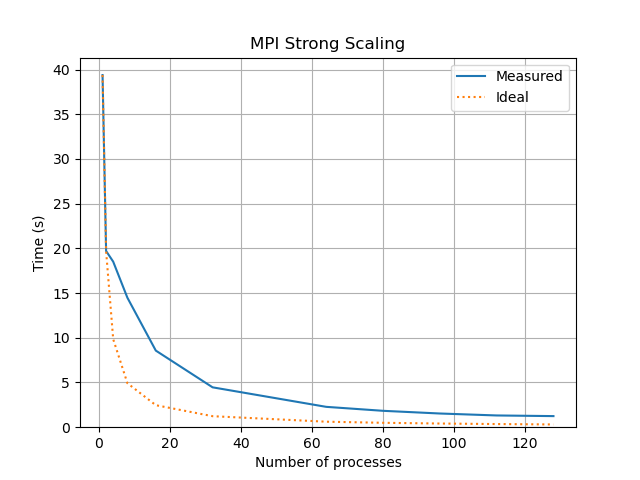
\includegraphics[width=0.8\textwidth]{../images/mpi_strong_scaling.png}
    \caption{MPI strong scaling}
    \label{fig:mpi_strong_scaling}
\end{figure}

\begin{figure}[h!]
    \centering
    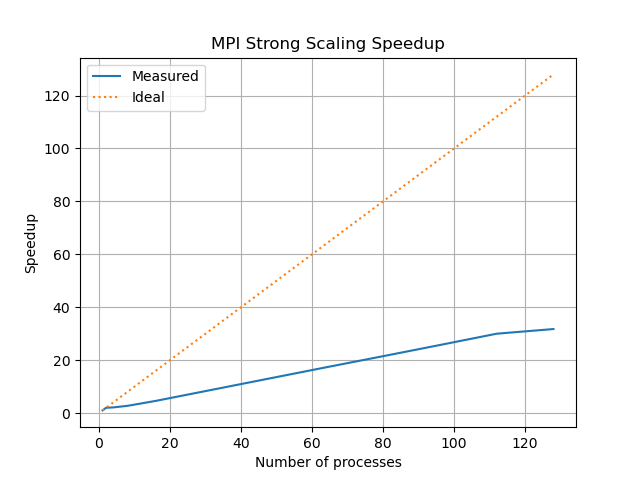
\includegraphics[width=0.8\textwidth]{../images/mpi_strong_scaling_speedup.png}
    \caption{MPI strong scaling speedup}
    \label{fig:mpi_strong_scaling_speedup}
\end{figure}


\begin{figure}[!h]
    \centering
    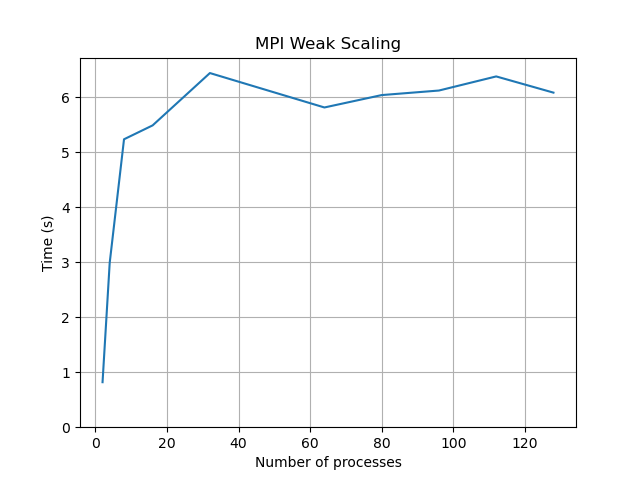
\includegraphics[width=0.8\textwidth]{../images/mpi_weak_scaling.png}
    \caption{MPI weak scaling}
    \label{fig:mpi_weak_scaling}
\end{figure}

\begin{figure}[h!]
    \centering
    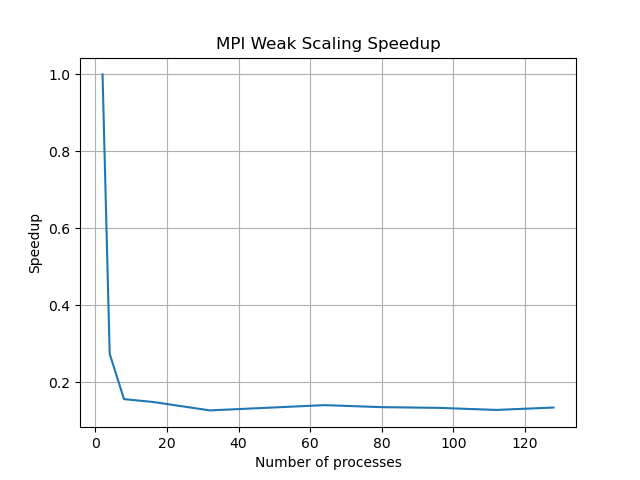
\includegraphics[width=0.8\textwidth]{../images/mpi_weak_scaling_speedup.png}
    \caption{MPI weak scaling speedup}
    \label{fig:mpi_weak_scaling_speedup}
\end{figure}


\subsection{OpenMP scaling}

The OpenMP strong scaling seems to scale with some more overhead than the MPI strong scaling. However, there is a substantial discrepancy between the ideal and the actual strong scaling as shown in Figure \ref{fig:openmp_strong_scaling}. After 20 threads the speedup decreases and becomes constant. This means that the overhead is significantly larger than the computation time.

For what concerns the OpenMP weak scaling, the speedup becames constant as the number of threads increases as shown in Figure \ref{fig:openmp_weak_scaling_speedup}. We can notice that in this case the scaling assumes a step-like shape. This is due to the fact that we decided to round the square root of the number of threads to the nearest integer to make the amount of work per thread appproximately harder.

\begin{figure}[h!]
    \centering
    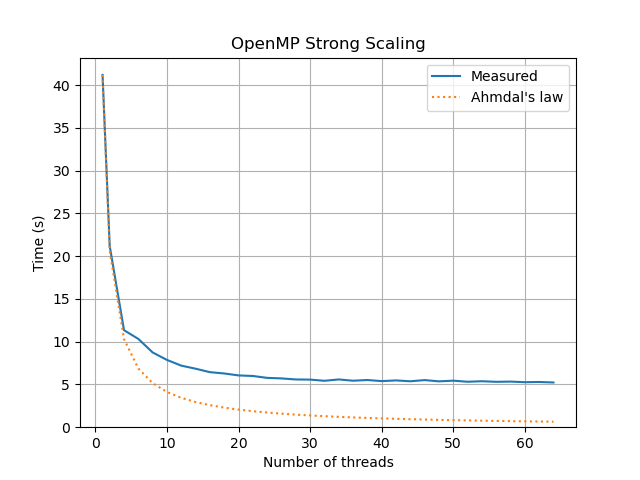
\includegraphics[width=0.8\textwidth]{../images/omp_strong_scaling.png}
    \caption{OpenMP strong scaling}
    \label{fig:openmp_strong_scaling}
\end{figure}

\begin{figure}[h!]
    \centering
    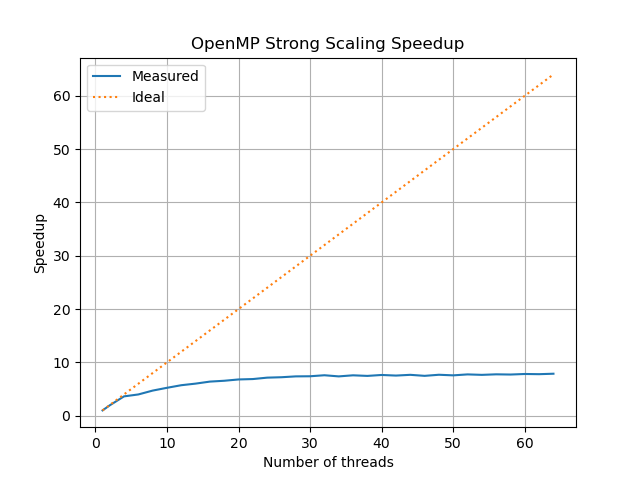
\includegraphics[width=0.8\textwidth]{../images/omp_strong_scaling_speedup.png}
    \caption{OpenMP strong scaling speedup}
    \label{fig:openmp_strong_scaling_speedup}
\end{figure}

\begin{figure}[h!]
    \centering
    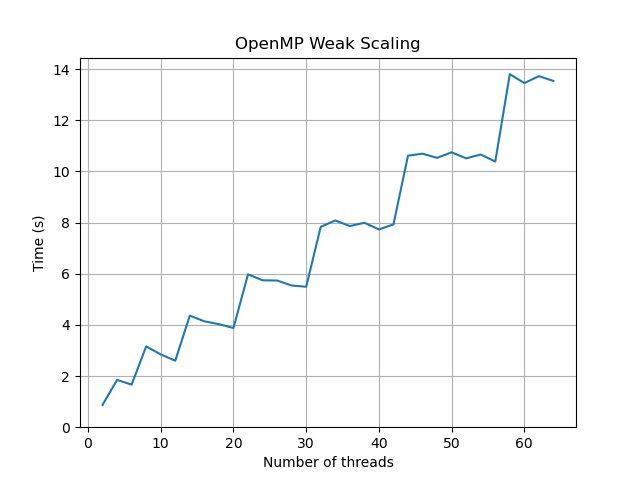
\includegraphics[width=0.8\textwidth]{../images/omp_weak_scaling.png}
    \caption{OpenMP weak scaling}
    \label{fig:openmp_weak_scaling}
\end{figure}

\begin{figure}[h!]
    \centering
    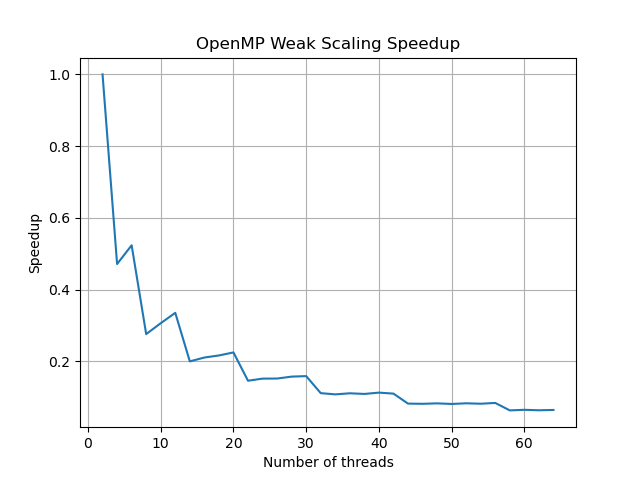
\includegraphics[width=0.8\textwidth]{../images/omp_weak_scaling_speedup.png}
    \caption{OpenMP weak scaling speedup}
    \label{fig:openmp_weak_scaling_speedup}
\end{figure}



